\chapter{AI-Greyboxing}
\label{cha:GreyBoxing}
Der erste Ansatz, der verfolgt wird, wird im Folgenden \textit{Greyboxing} genannt.
\section{Konzept}
\label{sec:KonzeptGreyBoxing}
Das Konzept ist hierbei, dass über einen Generator zufällige Nicht-Straßenbilder erzeugt werden, diese von der Schnittstelle bewertet werden, und eine zweite, lokale AI auf die Scores der Schnittstelle trainiert werden. 
~\newline
Mit fortschreitendem Experiment soll die lokale \ac{KI} ihr Verhalten an das der Schnittstelle angleichen und als Greybox dienen: Die lokal erzeugten Bilder und die lokalen Scores werden ähnlich zu den Scores der Schnittstelle. Ist dieser Zustand erreicht, kann man lokal Bilder generieren und sobald die GreyBox dieses akzeptiert an die Schnittstelle schicken. Die doppelt-bewerteten Ergebnisse können erneut ins Training einfließen, um die GreyBox weiter zu verbessern. 

Ausgehend hiervon können ebenfalls weitere Verbesserung am Generator vorgenommen und lokal getestet werden.
Man kann somit den Generator ebenfalls \textit{trainieren} und gegebenenfalls Hyperparamter wie Farbanteile oder Helligkeit anpassen. 

Das Konzept umfasst im erweiterten Sinn ebenfalls alle Maßnahmen, um die stetige, iterative Verbesserung der beteiligten Komponenten zu vollziehen. Als Generator wird für die Implementierung einfaches Rauschen gewählt. Andere mögliche Generatoren sind z.B. Webcrawler, welche Bilder nach gewissen Parametern aussuchen oder Generatoren, welche ein Bild lediglich \textit{verzerren} wie beim Verfahren der Degeneration, welches in Kapitel \ref{cha:Degeneration} erläutert wird. 

\section{Implementierung und erste Ergebnisse}\label{sec:ImplementierungGreyBoxing}

Die Abbildung \ref{fig:greyboxingstart} zeigt einen Überblick über die \textit{Setup-Phase} des Greyboxing:

\begin{figure}[h]
	\centering
	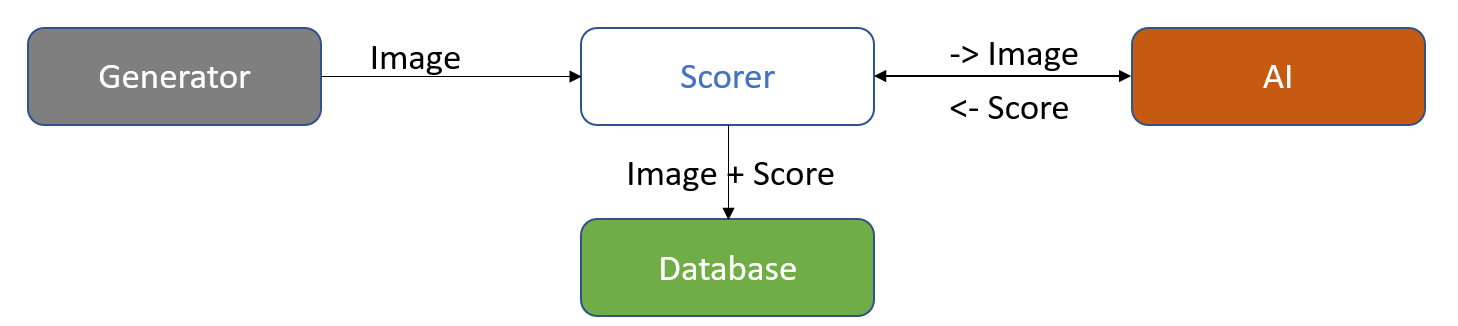
\includegraphics[width=0.9\linewidth]{Images/GreyBoxingStart}
	\caption[Komponenten Setup-Phase]{Komponenten Setup-Phase}
	\label{fig:greyboxingstart}
\end{figure}

\begin{itemize}
	\item \textbf{Generator:} Produziert zufällige Bilder auf Abruf. Innerhalb des ersten Ansatzes wird der Generator als einfaches Pythonfile mit wenigen Methoden umgesetzt.
	\item \textbf{Scorer:} Erhält Bilder vom Generator, lässt sie von der Schnittstelle bewerten und speichert die Ergebnisse samt Bild in einer Datenbank. Die Hauptlogik findet somit im Scorer statt. Er wurde als Jupyternotebook umgesetzt.
	\item \textbf{\ac{AI}:} Die Trasi-Schnittstelle, wie in Abschnitt \ref{sec:EigenschaftenTrasi} beschrieben.
	\item \textbf{Database:} Eine Datenbank, die Bilder und Scores abspeichert.
	In der Implementierung wird eine MongoDB gewählt, welche sich gut eignet um die JSON-Antworten der Schnittstelle direkt zu verwalten. 
\end{itemize}

Mit dieser Architektur werden über einen längeren Zeitraum knapp 100 000 Bilder gesammelt und abgespeichert. Nach der Sammlung der Daten wird eine \ac{KI} trainiert, welche die Scores der Schnittstelle imitiert. Hierfür wird das Framework Tensorflow gewählt und verschiedene Modell"-konfigurationen sowie Hyperparameter durchgespielt. 

Bei der praktischen Umsetzung zeigt sich, dass kein zufriedenstellendes Modell erzeugt werden kann. Eine detaillierte Ausführung dazu findet sich im nachfolgenden Abschnitt \ref{sec:ProblemGreyBoxing}.

Unabhängig davon soll noch einmal das Konzept nach dem Training vorgestellt werden, dargestellt in Abbildung \ref{fig:greyboxingrunning}: 
 \begin{figure}[h]
 	\centering
 	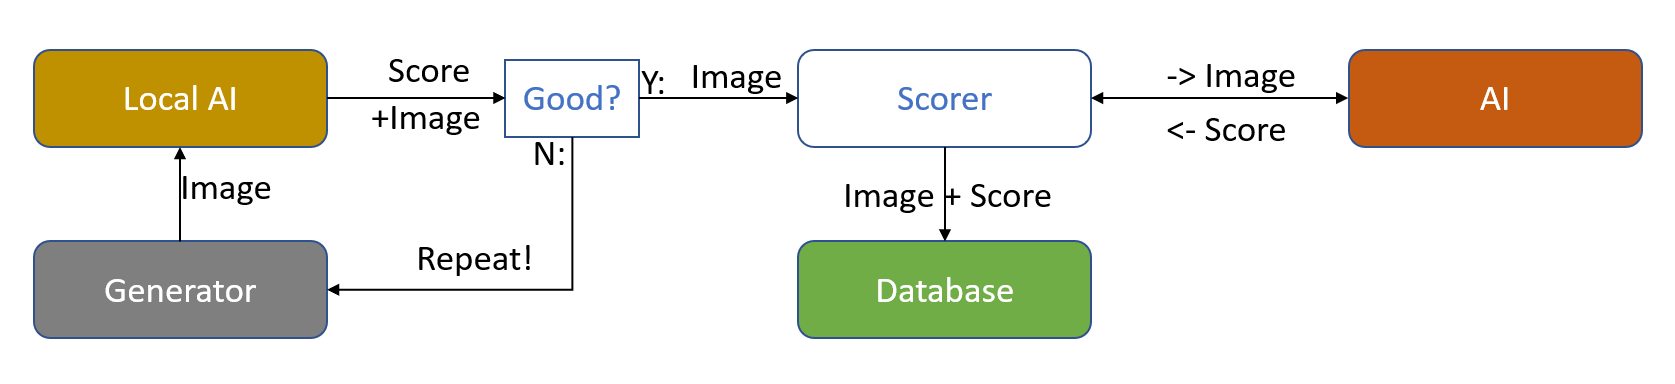
\includegraphics[width=0.9\linewidth]{Images/GreyBoxingRunning}
 	\caption{Komponenten Betriebs-Phase}
 	\label{fig:greyboxingrunning}
 \end{figure}
 Als neue Komponente ist die \textbf{lokale \ac{KI}} hinzugekommen, welche zunächst die Bilder des Generators prüft, und lediglich solche weitergibt, welche bereits von ihr als \textit{gut} eingestuft werden. 
 
Vorausgesetzt die lokale \ac{KI} erfüllt ihren Zweck, hilft sie iterativ mit jedem Bild eine bessere Datenmenge zu sammeln, bzw. innerhalb der Datenbank höhere Scores zu hinterlegen. Mit steigender Dauer und mehr Training sollte die lokale \ac{KI} somit immer bessere Ergebnisse erzielen. 
Weiterhin ist es denkbar, ein \textit{Ensemble} aus verschiedenen Klassifizieren zu etablieren, wobei der erste zwischen \textit{schlecht} und \textit{medium} entscheidet, der zweite zwischen \textit{medium} und \textit{gut} und die Kette nach diesem Muster fortgesetzt wird.
 
Ebenso hilft eine funktionierende lokale \ac{KI} direkt an dem Generator \textit{zu experimentieren}, um dort bessere Parameter zu erarbeiten. 
 
Als weiterführender Gedanke kann eine zusätzliche Komponente \textit{Generator-Tuner} kreiert werden, welche den Generator für die lokale \ac{KI} mit jedem erzeugten Bild \textit{optimiert}. Die Schwierigkeit dabei ist verschiedene Bilder zu erzeugen. 
 
Die Ähnlichkeit der lokalen \ac{KI} zur Schnittstelle kann direkt in der Datenbank gemessen werden: Jedes hinterlegte Bild eines Testsets wird ebenfalls von der lokalen \ac{KI} bewertet und der Score in der Datenbank erfasst. 
 Dieses Tripel aus \textit{<Bild, RemoteScores, LocalScores>} ermöglicht eine ganze Bandbreite von Ähnlichkeitsmaßen direkt in der Datenbank, von welcher aus sie performant abrufbar sind.  
\newpage
\section{Fehler- und Problemanalyse}
\label{sec:ProblemGreyBoxing}
Der Ansatz des \textit{Greyboxing} ist bereits in seiner Setup-Phase gescheitert. Zu betonen ist allerdings, dass er vor allem aus zeitlichen Aspekten verworfen wird, um zeitnah erfolgreiche Ergebnisse zu liefern.
~\newline
Grund für das frühe Ende ist das Training des lokalen neuronalen Netzes: Dieses kann bereits auf Basis der separierten Testdaten keine hinreichenden Scores erzielen. 

Im ersten Ansatz werden die Schnittstellen-Scores nach ihrem Prozentsatz mit einem Label versehen: \textit{Schwach} für einen Score <20\%, \textit{Medium} für einen Score >20\% und <50\% und \textit{Stark} für >50\%. Zunächst wird mit dem \textit{rohen Verhältnis} von 80:18:2 gearbeitet (Trainings- und Testsets mit entsprechendem Verhältnis), wobei die erzeugten Netze lediglich das Verhältnis erzeugen und in jedem Fall \textit{schwach} vorhergesagt haben. 

In einem zweiten Ansatz werden lediglich \textit{schwache} und \textit{medium} Bilder ausgewählt für das Training in einem 1:1 Verhältnis. Dieses neuronale Netz hat ebenfalls nur \textit{geraten} und erreichte eine Accuracy von 50\%. Ein möglicher und wahrscheinlicher Grund für diesen Wert ist die Zufälligkeit der Bilder, bzw. die Verschiedenheit der einzelnen Bilder zueinander. Diese ist ebenfalls zufällig. Für das nicht trainierte Netz besitzen die Bilder keinen Zusammenhang zu ihrem Label. Diese Zuordnung erscheint dem Netz ebenfalls zufällig. Innerhalb der Back-Propagation \cite{zhou_understanding_2018} werden nun die Gewichte angezogen, damit das zufällige Bild bei einem erneuten Durchlauf einen erhöhten Score erzielt. Da das zugrundeliegende Bild allerdings nur aus Rauschen besteht, wird im Wesentlichen nur ein (verringertes) Rauschen auf die Gewichte des Netzes angewandt. De facto hat das Netz also nichts gelernt, sondern sich nur etwas verformt. 

In genauerer Betrachtung \textit{schrumpfen} die Gewichte des Netzes und lediglich der Bias der Ausgabeschicht ist ausschlaggebend für das Ergebnis der Klassifikation. Der Bias entspricht mit fortschreitendem Training dem höchsten Verhältnis innerhalb der Trainingsmenge.

\paragraph{Mögliche Lösungsansätze}~\newline
Zwei mögliche Lösungsansätze sind die Verwendung eines nicht-zufällig initialisierten Netzes via Transfer Learning \cite{5288526} oder die Verwendung eines weniger zufälligen Generators. Ein transferiertes Netz kann hierbei seine ersten Layer, welche Features extrahieren und z.B. Kanten erkennen, behalten, und lediglich die hinteren Schichten dafür nutzen das Verhalten der Schnittstelle nachzuahmen. Innerhalb dieses Ansatzes ist es unabdingbar, dass die ersten Schichten des Netzes \textbf{nicht} trainiert bzw. verändert werden, sondern ihre Funktionalitäten behalten. 

Als alternative Generatoren bieten sich solche an, welche \textit{Formen} generieren: Streifen, Kugeln oder \textit{echte} Bilder. Die Verwendung eines solchen Generators hat zur Folge, dass die Bilder im Trainingsset nicht vollständig zufällig sind, sondern im Wesentlichen durch ihre Formen definiert sind. Das Netz ist somit im Stande auf jeden Fall Formen zu erkennen und diese zu gewichten und zu bewerten. Als Variante hiervon eignen sich Webcrawler-Generatoren, welche z.B. geeignete Katzenbilder aus dem Internet suchen.   